% Owner: Sharjeel Shahid 24L-3055
\section{Deep Learning Model (PyTorch)}
\label{sec:deep}

\subsection{Framework and Motivation}
PyTorch provides automatic differentiation, recurrent layers and an explicit training loop, which makes the sequence construction, loss calculation and checkpoint selection easy to inspect~\cite{b_paszke2019pytorch}. The long short-term memory (LSTM) network maintains a recurrent state over the input sequence~\cite{a_hochreiter1997}. It can therefore use how the features evolved over the last $L$ trading days. The classical models receive one engineered row at a time, although that row already contains lagged features. This is a different representation of temporal information, not a guarantee that the LSTM will outperform those models.

Decimal metrics in this section and Section~\ref{sec:error-bias} are truncated towards zero at the displayed precision; counts and configuration values are exact.

\subsection{Input Windows}
% Sources: models/deep/lstm_config.json; src/deep/dataset.py; prediction CSV row counts.
The saved final configuration uses $L=60$ trading days and $F=14$ stationary features, giving an input tensor of shape $[\mathrm{batch},60,14]$. The label is \texttt{direction\_5d} on the last day of the window: whether gold is higher after the following five trading days. Neither \texttt{direction\_5d} nor the future price \texttt{gold\_5d\_ahead} is an input feature.

The split remains chronological: training covers 2010--2021, validation covers 2022--2023, and testing covers 2024--2026. A validation window can borrow the final $L-1=59$ feature rows of training; a test window can borrow the corresponding rows of validation. These are observations from earlier dates, and their labels are not borrowed. This past-only context gives a prediction for every validation and test date without introducing future input features. The prediction file contains 2,929 training rows from 2,988 available training rows, followed by 502 validation rows and 701 test rows. Training loses its first 59 rows because no complete earlier window exists. Batches of training windows are shuffled, but neither split membership nor the chronological order within a window changes.

The \texttt{all} feature set contains 27 features. The \texttt{stationary} alternative removes the designated price-level features and retains 14 features. This choice reduces direct dependence on levels whose test-period distribution is far from the training distribution; Section~\ref{sec:error-bias} quantifies this for scaled gold. The name \texttt{stationary} describes the selected feature subset, rather than establishing statistical stationarity of every retained series. Both alternatives use the existing preprocessing fitted on training data.

\subsection{Architecture}
\begin{figure}[H]
    \centering
    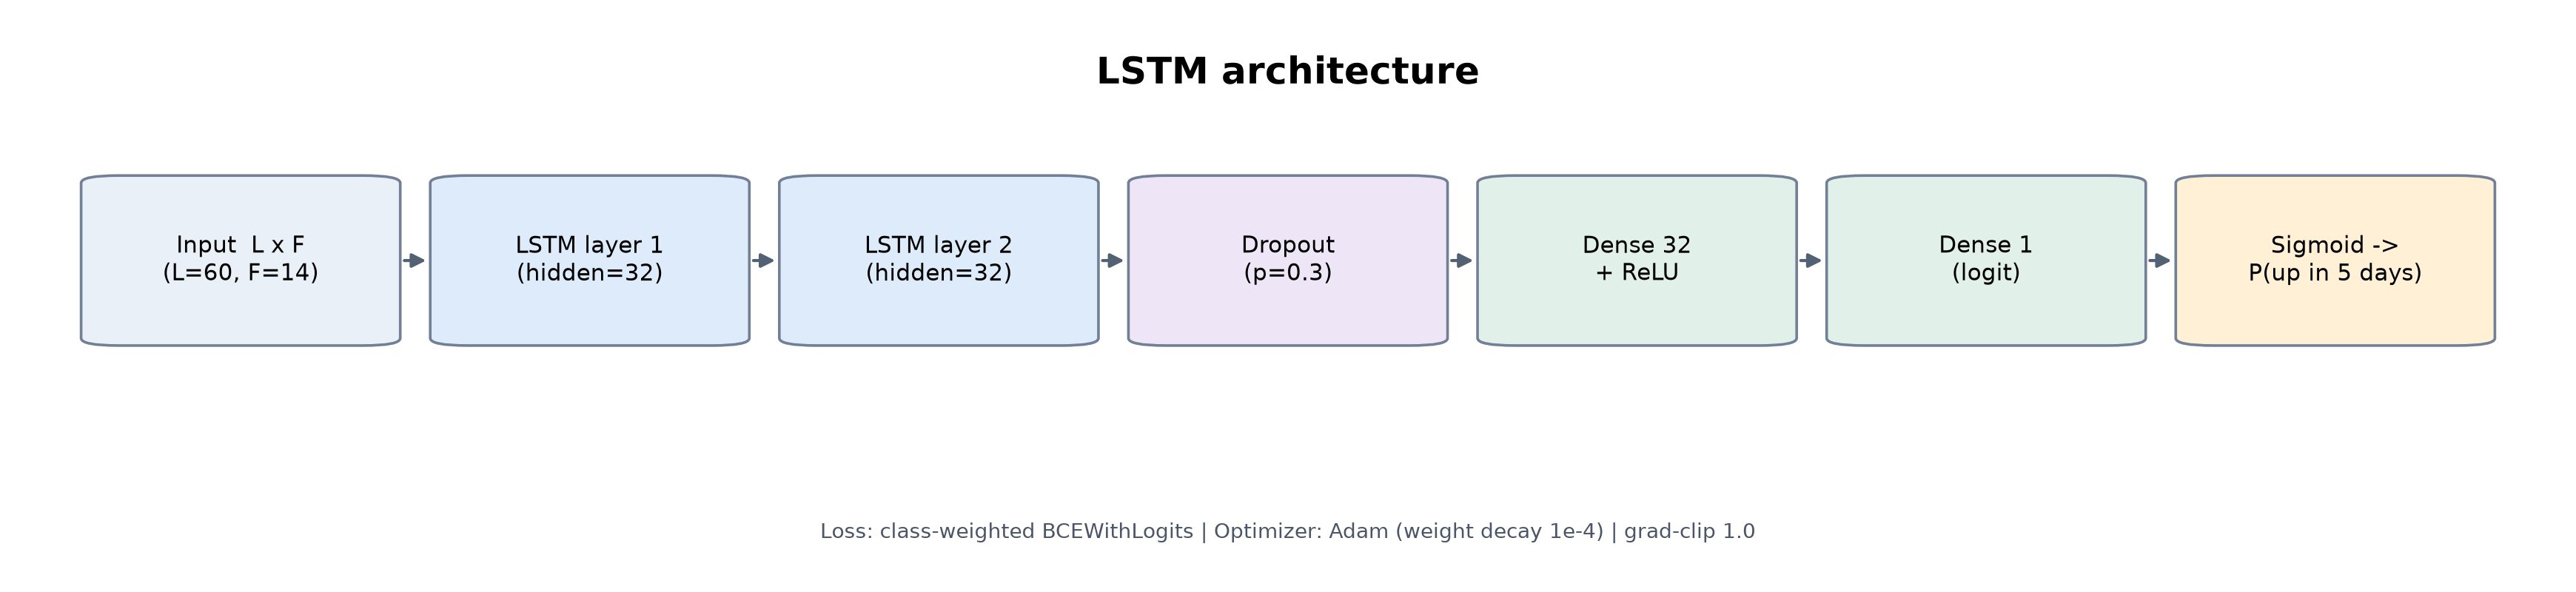
\includegraphics[width=\textwidth]{deep/lstm_architecture.png}
    \caption{Architecture of the final LSTM. The sigmoid shown after the output is used for prediction; the model itself returns a logit.}
    \label{fig:b-deep-architecture}
\end{figure}

% Source: src/deep/model.py; configuration above; parameter count from model.parameters().
Two stacked LSTM layers each have hidden size 32. Dropout with probability 0.3 is applied between the recurrent layers. The output at the last time step passes through a separate dropout layer with probability 0.3, a dense layer with 32 outputs, a ReLU, and a dense layer with one output. Dropout is intended to reduce overfitting by randomly suppressing activations during training~\cite{b_srivastava2014dropout}; it is disabled during evaluation. Instantiating the implemented model with the final configuration gives exactly 15,681 trainable parameters.

The final scalar is a logit, not a probability. The sigmoid is applied when generating probabilities and is incorporated into the loss calculation. This avoids placing a separate sigmoid inside the model before a loss that already handles it.

\subsection{Loss and Optimizer}
% Sources: train_lstm.py and model.py; lstm.csv train labels after removing its last HORIZON=5 rows.
The fitting dataset purges the last five training windows because their labels look beyond the training boundary. Starting with the unpurged training predictions, dropping these five final dates leaves 2,924 labels: 1,345 down labels and 1,579 up labels. The class weight is therefore
\[
    \mathrm{pos\_weight}
    = \frac{\#\{y=0\}}{\#\{y=1\}}
    = \frac{1345}{1579}
    = 0.851804\ldots .
\]
This value is passed as a float32 tensor to \texttt{BCEWithLogitsLoss}. It scales the positive-class contribution relative to the negative-class contribution. The combined sigmoid and binary cross-entropy calculation is numerically more stable than explicitly converting extreme logits to probabilities before evaluating the loss.

Adam~\cite{b_kingma2015adam} uses a learning rate of 0.001, a batch size of 32, and weight decay $10^{-4}$ to penalise large weights. Before each update, the total gradient norm is clipped at 1.0 to limit large recurrent-network gradients~\cite{b_pascanu2013clipping}. The Python, NumPy and PyTorch random seeds are all 42, and training runs on the CPU.

Unlike the training split, validation is not purged in the implemented loader. This preserves all validation predictions, but the final five validation labels can use prices from the test calendar period. Thus past-only input context prevents feature leakage, while the unpurged validation boundary remains a limitation of model selection.

\subsection{Hyperparameter Tuning}
% Sources: results/tuning/lstm_tuning.csv and src/deep/tune_lstm.py.
Each configuration uses two recurrent layers, at most 100 epochs, and early-stopping patience of 10 epochs. Within a run, validation loss determines the checkpoint. Between runs, the highest validation AUC at that checkpoint determines the selected configuration; no test metric is used. Ties use lower validation loss when available, then grid order.

\begin{table}[H]
    \centering
    \small
    \begin{tabular}{lrrrrrr}
        \toprule
        Features & Window & Hidden & Dropout & LR & Batch & Val. AUC \\
        \midrule
        all        & 20 & 32 & 0.1 & 0.001 & 32 & 0.3879 \\
        stationary & 20 & 32 & 0.1 & 0.001 & 32 & 0.5424 \\
        all        & 60 & 32 & 0.1 & 0.001 & 32 & 0.4448 \\
        stationary & 60 & 32 & 0.1 & 0.001 & 32 & 0.5323 \\
        all        & 20 & 64 & 0.1 & 0.001 & 32 & 0.5001 \\
        stationary & 20 & 64 & 0.1 & 0.001 & 32 & 0.4820 \\
        all        & 60 & 64 & 0.1 & 0.001 & 32 & 0.4941 \\
        stationary & 60 & 64 & 0.1 & 0.001 & 32 & 0.5580 \\
        all        & 20 & 32 & 0.3 & 0.001 & 32 & 0.4365 \\
        stationary & 20 & 32 & 0.3 & 0.001 & 32 & 0.5193 \\
        all        & 60 & 32 & 0.3 & 0.001 & 32 & 0.4585 \\
        \textbf{stationary} & \textbf{60} & \textbf{32} & \textbf{0.3} & \textbf{0.001} & \textbf{32} & \textbf{0.5934} \\
        all        & 20 & 64 & 0.3 & 0.001 & 32 & 0.5149 \\
        stationary & 20 & 64 & 0.3 & 0.001 & 32 & 0.4906 \\
        all        & 60 & 64 & 0.3 & 0.001 & 32 & 0.4780 \\
        stationary & 60 & 64 & 0.3 & 0.001 & 32 & 0.5429 \\
        all        & 20 & 32 & 0.1 & 0.001 & 64 & 0.4277 \\
        \bottomrule
    \end{tabular}
    \caption{All evaluated LSTM configurations in saved grid order. The selected row is bold. Each AUC comes from a single seeded run.}
    \label{tab:b-deep-grid}
\end{table}

Only 17 of the 64 planned configurations appear in the saved table: the grid was stopped early because of time. Every evaluated run uses learning rate 0.001, so the planned rate 0.0003 is untested. Both windows (20 and 60), feature sets (\texttt{all} and \texttt{stationary}), hidden sizes (32 and 64), and dropout probabilities (0.1 and 0.3) appear. However, 16 runs use batch size 32 and only one uses batch size 64; the combinations involving that larger batch are therefore mostly unevaluated.

Every configuration is a single run with seed 42. Differences of a few thousandths of AUC should be treated as potentially within run-to-run or sampling noise; that uncertainty was not measured. The selected stationary configuration has the largest recorded validation AUC, 0.5934, and is a defensible choice among the evaluated candidates. Its AUC is nevertheless an optimistic maximum over configurations assessed on one validation period, not an unbiased estimate of future performance.

% Download provenance and the reason for stopping are supplied by the project author; the saved selected AUC matches the final config.
Tuning used an earlier data download and only the final model was retrained on the frozen shared dataset; the training and validation rows are identical, so the selected configuration's validation result is unchanged, while only the test period differs.

\subsection{Training Behaviour}
% Source: results/history/lstm_history.csv; argmin(val_loss), first and last epoch numbering.
Training ran for 15 epochs. The best checkpoint was epoch 5, with validation loss 0.635452; the next 10 epochs did not improve it. Early stopping restores the epoch-5 weights before saving predictions. The history evaluates both training and validation in evaluation mode with the same class-weighted loss. Its training metrics cover the purged fitting dataset, whereas the prediction CSV retains the additional final training windows.

\begin{table}[H]
    \centering
    \small
    \begin{tabular}{lrrrrr}
        \toprule
        Checkpoint & Epoch & Train loss & Val. loss & Train acc. & Val. acc. \\
        \midrule
        Best & 5  & 0.629206 & 0.635452 & 0.5526 & 0.5816 \\
        Last & 15 & 0.494182 & 0.827428 & 0.7356 & 0.5139 \\
        \bottomrule
    \end{tabular}
    \caption{Evaluation-mode history at the best and last epochs. The last checkpoint is not used for the final predictions.}
    \label{tab:b-deep-history}
\end{table}

\begin{figure}[H]
    \centering
    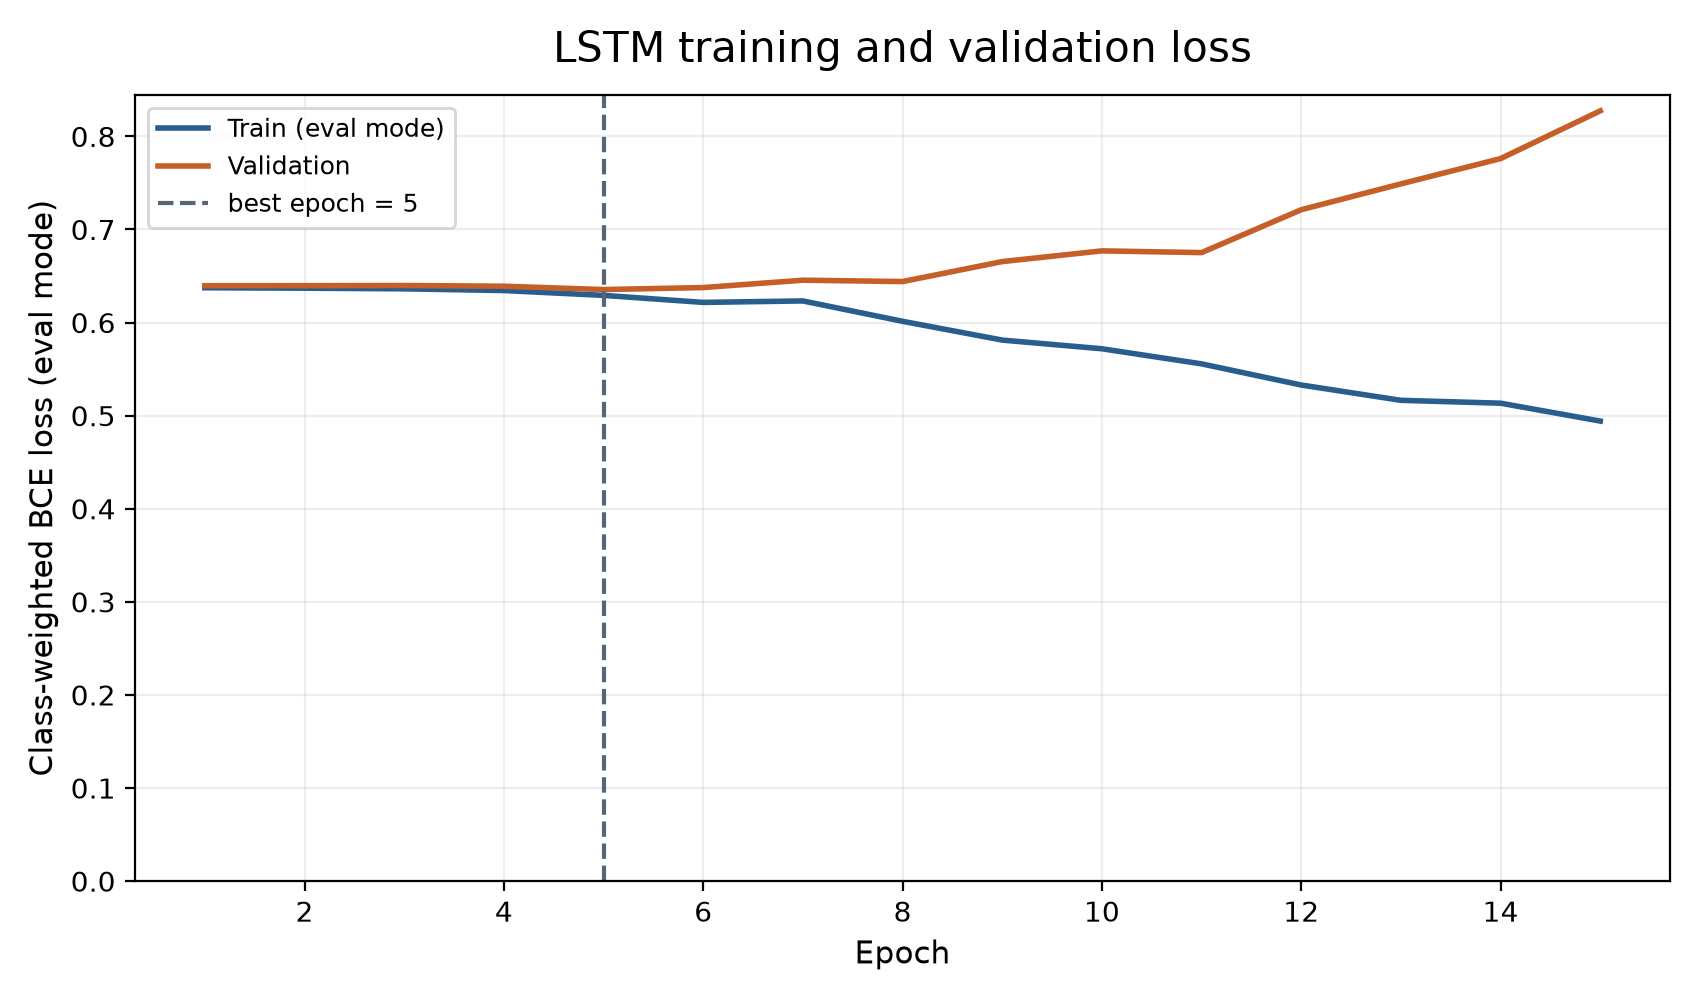
\includegraphics[width=0.88\textwidth]{deep/lstm_loss_curve.png}
    \caption{Class-weighted training and validation losses. The vertical line marks the minimum validation loss, which determines the restored checkpoint.}
    \label{fig:b-deep-loss}
\end{figure}

\begin{figure}[H]
    \centering
    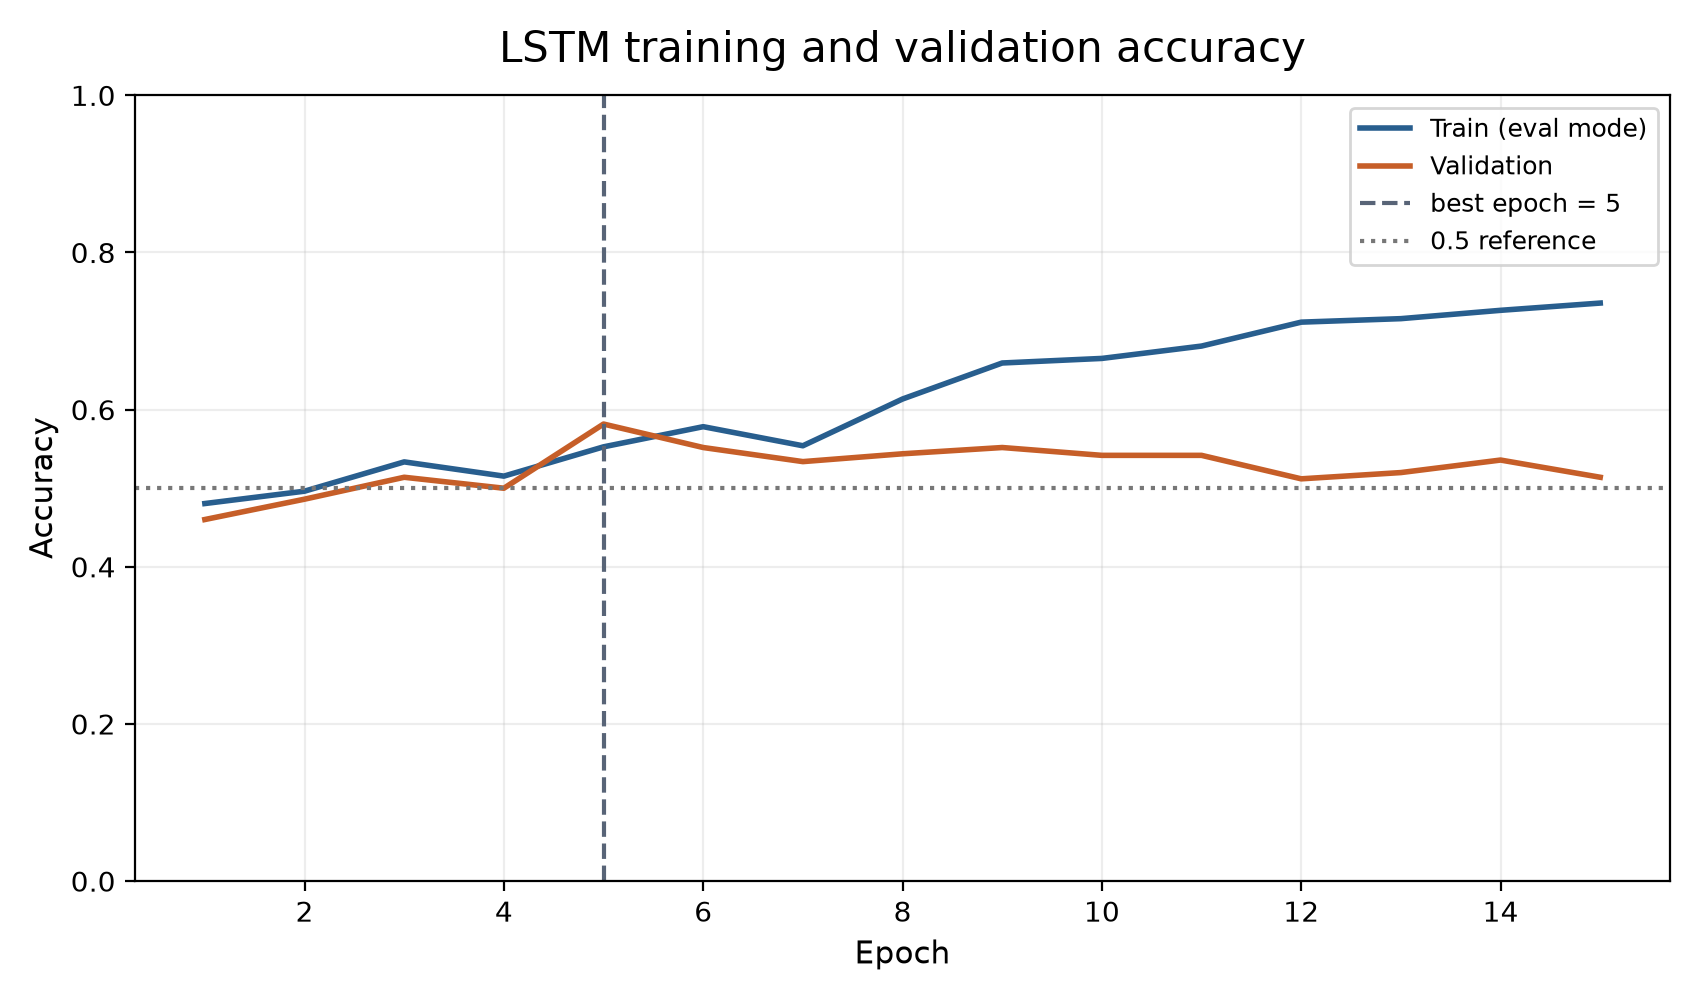
\includegraphics[width=0.88\textwidth]{deep/lstm_accuracy_curve.png}
    \caption{Training and validation accuracy in evaluation mode. The dotted horizontal line is the 0.5 reference, not the empirical majority baseline.}
    \label{fig:b-deep-accuracy}
\end{figure}

After the best epoch, training loss falls overall while validation loss rises, with fluctuations rather than a strictly monotonic trend. Training accuracy improves while validation accuracy deteriorates. These curves are consistent with overfitting to the fitting period and explain the need to restore the earlier checkpoint.

\subsection{Result Summary}
% Sources: saved config (validation AUC); bias_check.csv, model=lstm, split=test.
The final model's validation AUC is 0.5935. On the frozen test data, its accuracy is 0.5221, its predicted up-rate is 0.4593, and the true up-rate is 0.6091. It therefore falls below the always-up baseline accuracy of 0.6091 (Section~\ref{sec:evaluation}), despite avoiding the complete class collapse discussed in Section~\ref{sec:error-bias}.

On the shared test period (701 days) the final LSTM reaches a ROC-AUC of 0.5377, an F1 score of 0.5527, a precision of 0.6429 and a recall of 0.4848. The drop from the validation AUC of 0.5935 shows that the validation figure is optimistic, as it is the maximum over the evaluated configurations on a single period. A test AUC of 0.54 is only slightly above the 0.5 of a random ranking, so the model carries at most a weak directional signal. We therefore do not claim that the LSTM is useful for trading; it is mainly notable for not collapsing to a single class. These results do not establish a profitable trading strategy.